\documentclass{article}
\usepackage[english]{babel}
\usepackage{etoolbox}
\usepackage{pgfplots}
\usetikzlibrary{arrows}
\usepackage[utf8]{inputenc}
\usepackage[margin=0.5in]{geometry}
\usepackage{bbold}
\usepackage{amsmath}
\usepackage{graphicx}
\usepackage{amsmath}
\usepackage[makeroom]{cancel}
\graphicspath{ {./images/} }
\renewcommand{\arraystretch}{3}
\usepackage{xcolor}
\setlength\parindent{0pt}
\newcommand*{\Perm}[2]{{}^{#1}\!P_{#2}}%
\newcommand*{\Comb}[2]{{}^{#1}C_{#2}}%

\title{Fourier Series Question - \zeta(4)}
\author{David Veitch}
\date{November 2018}

\begin{document}

\maketitle

\section{Question}

Evaluate $\zeta(4)$ (where $\zeta$ is the Riemann Zeta function, $\zeta(s)=\sum_{n=1}^{\infty}\frac{1}{n^s}$, $s>1$) using the Fourier Series of $x^2$ for $-\pi < x < \pi$ and Parseval's Identity.
\section{Answer}
We first notice that $f(x)=x^2$ is an even function on $[-\pi,\pi]$ therefore its Fourier Series is given by a Fourier Cosine Series:\\
\begin{equation} 
\begin{split}
f(x) &= a_0 + \sum_{n=1}^{\infty}a_n\cos(\frac{n\pi x}{L}) = a_0 + \sum_{n=1}^{\infty}a_n\cos(\frac{n\pi x}{\pi}) = a_0 + \sum_{n=1}^{\infty}a_n\cos(nx)\\
\end{split}
\end{equation}

The coefficients for the Fourier Cosine Series, $a_0$ and $a_n$ are given by:
\begin{equation} 
\begin{split}
a_0 &= \frac{1}{L}\int_{0}^{L}f(x)dx = \frac{1}{\pi}\int_{0}^{\pi}x^2dx = \frac{x^3}{3\pi}\Big|_0^\pi = \frac{\pi^2}{3}\\
a_n &= \frac{2}{L}\int_{0}^{L}f(x)\cos(\frac{n\pi x}{L})dx \\
a_n &= \frac{2}{\pi}\int_{0}^{\pi}x^2\cos(nx)dx \quad \text{(Integrate By Parts)}\\
u=x^2 \quad du=2x& \quad v=\frac{1}{n}\sin(nx) \quad dv=\cos(nx)\\
a_n &= \frac{2}{\pi}\bigg(\Big[\frac{x^2}{n}\sin(nx)\Big]\Big|_0^\pi - \int_{0}^{\pi}\frac{2x}{n}\sin(nx)\bigg) \\
a_n &= \frac{2}{\pi}\bigg(0 - \int_{0}^{\pi}\frac{2x}{n}\sin(nx)\bigg)\\
a_n &= -\frac{4}{\pi n}\bigg(\int_{0}^{\pi}x\sin(nx)\bigg) \quad \text{(Integrate By Parts)}\\
u=x \quad du=1& \quad v=-\frac{1}{n}\cos(nx) \quad dv=\sin(nx)\\
a_n &= -\frac{4}{\pi n}\bigg(\big[-\frac{x}{n}\cos(nx)\big]\Big|_0^\pi + \int_{0}^{\pi} \frac{1}{n}\cos(nx)\bigg)\\
a_n &= -\frac{4}{\pi n}\bigg(-\frac{\pi}{n}\cos(\pi n) + \big[\frac{1}{n^2}\sin(nx)\big]\big|_0^\pi\bigg)\\
a_n &= -\frac{4}{\pi n}\bigg(-\frac{\pi}{n}\cos(\pi n) + 0\bigg)\\
a_n &= \frac{4}{n^2}\cos(\pi n)\\
a_n &= \frac{4(-1)^n}{n^2} \quad \text{(using fact $\cos(\pi n)=(-1)^n$)}
\end{split}
\end{equation}

\newpage We can then write the Fourier Series as:
\begin{equation} 
\begin{split}
f(x)=x^2=\frac{\pi^2}{3}+\sum_{n=1}^{\infty}\frac{4(-1)^n}{n^2}\cos(nx) \quad x\in [-\pi,\pi]\\
\end{split}
\end{equation}

Since $f(x)=x^2$ and $f'(x)=2x$ are piecewise continuous on $[-\pi,\pi]$ we can use Parseval's Equality: 
\begin{equation} 
\begin{split}
\frac{1}{L}\int_{-L}^{L}f(x)^2dx&=2a_0^2+\sum_{n=1}^{\infty}(a_n^2+b_n^2)\\
\frac{1}{\pi}\int_{-\pi}^{\pi}(x^2)^2dx&=2(\frac{\pi^2}{3})^2+\sum_{n=1}^{\infty}\bigg(\frac{4(-1)^n}{n^2}\bigg)^2\\
\frac{x^5}{5\pi}\big|_{-\pi}^{\pi} &= \frac{2\pi^4}{9}+\sum_{n=1}^{\infty}\frac{16(-1)^{2n}}{n^4}\\
\frac{2\pi^4}{5} - \frac{2\pi^4}{9} &= \sum_{n=1}^{\infty}\frac{16}{n^4} \quad \text{(since $(-1)^{2n}=1$)}\\
\frac{\pi^4}{90} &= \sum_{n=1}^{\infty}\frac{1}{n^4}
\end{split}
\end{equation}

Therefore we conclude that

\begin{equation} 
\begin{split}
\zeta(4) &= \sum_{n=1}^{\infty}\frac{1}{n^4} = \frac{\pi^4}{90}
\end{split}
\end{equation}

\newpage

\section{Supplemental Material}

Wow what a result! There is something extraordinary about finding the value of an equation that never terminates. The Riemann Zeta function can be evaluated at other values as well (for example $\zeta(2)=\frac{\pi^2}{6}$).\\

Graph of the Fourier Series of $x^2$ for $x \in [-\pi,\pi]$:\\

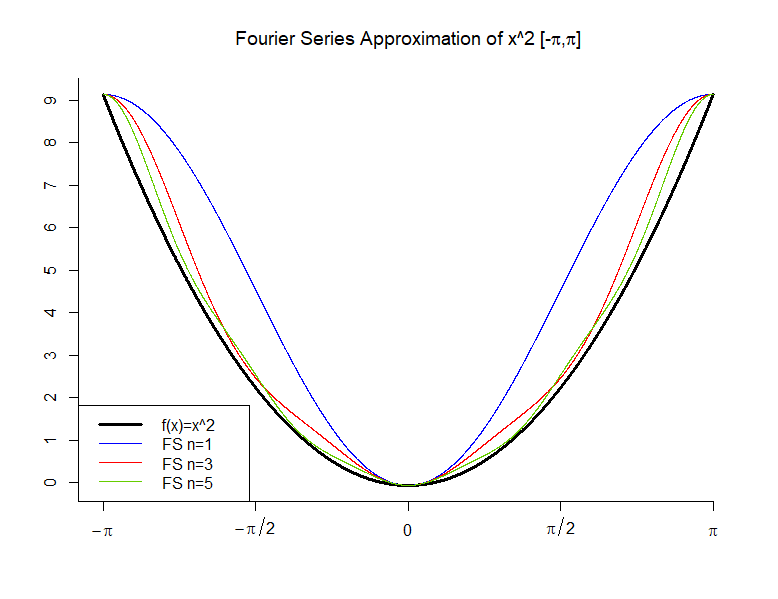
\includegraphics[width=\textwidth]{Rplot.png}

Special thanks to Aghil Alaee who assigned this question as a homework question for APM346 Partial Differential Equations at the University of Toronto in the summer of 2018.

\end{document}
